\section{Implementation and evaluation}\label{sec:experiment}
In this section, an experimental evaluation over six real-life event logs is reported.
The aim of the evaluation is to measure to what extent the forecasted process models/DFGs are capable of correctly reproducing actual future DFGs in terms of allowing for the same process model behaviour.
To this purpose we benchmark the actual against the forecasted entropic relevance discussed in \Cref{sec:2:motivation}.
This is done at various parts of the trace, i.e. forecasts for the middle of the event logs up to the later parts of the event log to capture the robustness of the forecasting techniques in terms of the amount of data required to obtain good prediction results for both the equisized and equitemporal aggregation.

\subsection{Re-sampling and test setup}
To obtain training data, time series are obtained by specifying a number of intervals (i.e. time steps in the DF time series) using either equitemporal or equisized aggregation a described in Section \ref{sec:3a:preliminaries}.
Time series algorithms are parametric and sensitive to sample size requirements \cite{hanke2001business}.
Depending on the number of parameters a model uses, a minimum size of at least 50 steps is not uncommon, although typically model performance should be monitored at a varying number of steps.
In the experimental evaluation, the event logs are divided into 100 time intervals with a varying share of training and test intervals. A constant and long horizon $h=25$ is used meaning all test sets contain 25 intervals, but the training sets are varied from $ts=25$ to $ts=75$ intervals, meaning the forecasts progressively target the prediction of intervals 25-50 (the second quarter of intervals) over to 75-100 (the last quarter of intervals).
This allows to both inspect the difference in results when only few data points are used, and whether there is a difference forecasting data points in the middle or towards the end of the available event data.

Resampling is applied based on a 10-fold cross-validation constructed following a rolling window approach for all horizon values $h\in[1,25]$ where a recursive strategy is used to iteratively obtain $\hat{y}_{t+h|T_{t+h-1}}$ with $(y_1,\dots,y_{T},\dots,\hat{y}_{t+h-1})$ \cite{weigend2018time}.
10 training sets are hence constructed for each training set length $ts$ and exist from $(y_1,\dots,y_{T-h-f})$ and the test sets from $(y_{T-h-f+1},\dots,y_{T-f})$ with $f\in[0,9]$ the fold index \cite{bergmeir2012use}.
While direct strategies with a separate model for every value of $h$ can be used as well and avoid the accumulation of error, they do not take into account statistical dependencies for subsequent predictions.

Three popular publicly-available event logs are used: the BPI challenge of 2012 log\footnote{\url{https://doi.org/10.4121/uuid:3926db30-f712-4394-aebc-75976070e91f}}, 2017\footnote{\url{https://doi.org/10.4121/uuid:5f3067df-f10b-45da-b98b-86ae4c7a310b}}, and 2018\footnote{\url{https://doi.org/10.4121/uuid:3301445f-95e8-4ff0-98a4-901f1f204972}}, the Sepsis cases event log\footnote{\url{https://doi.org/10.4121/uuid:915d2bfb-7e84-49ad-a286-dc35f063a460}}, an Italian help desk log\footnote{\url{https://doi.org/10.4121/uuid:0c60edf1-6f83-4e75-9367-4c63b3e9d5bb}}, and the Road Traffic Fine Management Process log (RTFMP) event log (see Section \ref{sec:2:motivation}).
Each of these logs has a diverse set of characteristics in terms of case and activity volume, as well as average trace length, as can be seen in Table \ref{tab:eventlogs}.
\begin{table}[htbp]
  \centering
  \resizebox{0.6\textwidth}{!}{
    \begin{tabular}{lrrr}
    \toprule
    \textbf{Event log} & \multicolumn{1}{l}{\textbf{\# cases}} & \multicolumn{1}{l}{\textbf{\# activities}} & \multicolumn{1}{l}{\textbf{Average trace length}} \\
    \midrule
    \textbf{BPI 12} & 13,087 & 36    & 20.02 \\
    \textbf{BPI 17} & 31,509 & 26    & 36.83 \\
    \textbf{BPI 18} & 43,809 & 170   & 57.39 \\
    \textbf{Sepsis} & 1,050 & 16    & 14.49 \\
    \textbf{RTFMP} & 150,370 & 11    & 3.73 \\
    \textbf{Italian} & 4,580 & 14    & 4.66 \\
    \bottomrule
    \end{tabular}%
    }
  \caption{Overview of the characteristics of the event logs used in the experimental evaluation.}
  \label{tab:eventlogs}%
\end{table}%

%An example of applying the equisized or equitemporal aggregation to the Sepsis event log with 100 intervals results in the DF time series of Figure \ref{fig:sepsists}, where the DF occurrences of the most frequently occurring activity pair is included.
%For the equisized aggregation, the number of DFs is indeed relatively stable over the log's timeline where for the equitemporal aggregation a noticeable decline of DF pairs is visible towards the end of the series.
%This phenomenon is typical in event logs, as processes usually have particular endpoint activities, but can also be due to the unequal distribution of events over the event log's time line.
There are a few considerations concerning the DF time series in these event logs.
Firstly, DFs of activity pairs containing end point activities (i.e. at the start/end of a trace) often only contain meaningful numbers at very particular parts of the series and are hard to process by longitudinal algorithms which require a longer pattern to extract a meaningful pattern for prediction.
Secondly, especially the equitemporal aggregation can suffer from event logs in which events do not occur as frequently throughout the full log's development.
E.g., the Sepsis log's number of event occurrences tails off towards the end which can be alleviated by pre-processing (not done here to remain consistent over the event logs).
Finally, if the level of occurrences of the DF pair is low and close to 0, the series might be too unsuitable for analysis with white noise series analysis techniques that assume stationarity.
Ideally, every time series is tested using a stationarity test such as the Dickey-Fuller unit root test \cite{leybourne1995testing} and an appropriate lag order is established for differencing. 
Furthermore for each algorithm, especially ARIMA-based models, (partial) auto-correlation could establish the ideal $p$ and $q$ parameters.
However, for the sake of simplicity and to avoid solutions where each activity pair has to have different parameters, various values are used for $p$, $d$, and $q$ and applied to all DF pairs where only the best-performing are reported below for comparison with the other time series techniques.
The results contain the best-performing representative of each forecasting family.
% \begin{figure}[tb]
% 	\centering
% 	\subfigure[Most common DF - equisize]{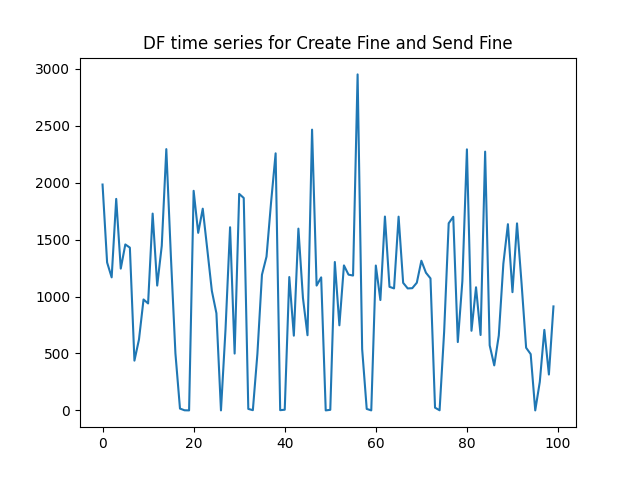
\includegraphics[width=0.39\textwidth]{./img/rtfmp_1.png}}
% 	\subfigure[Most common DF - equitemp]{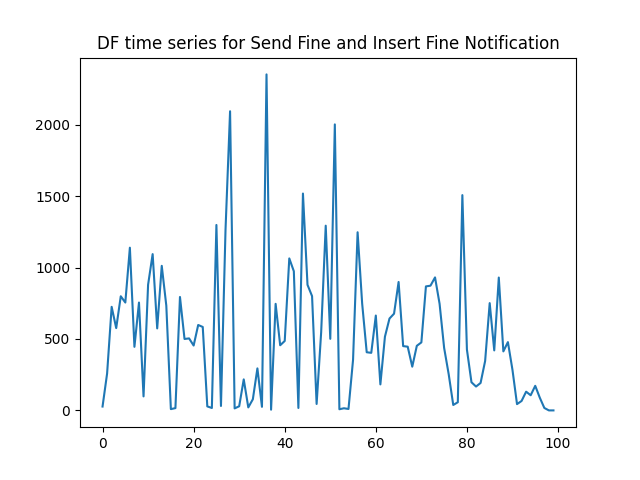
\includegraphics[width=0.39\textwidth]{./img/rtfmp_1_t.png}}
% 	\caption{RTFMP}
% 	\label{fig:sepsists}
% \end{figure}

% \subsection{Evaluation criteria}
% Given that we want to evaluate the capability of the approach to accurately predict the evolution of the process model, the combination of all DF predictions is considered to obtain a global DFG prediction.
% The following two criteria are used:
% \begin{itemize}
% 	\item \textbf{Cosine distance:} measures the distance between two vectors and is often used to compare graph distance. This metric is used to compare the DFGs' edge weight matrices between the actual and predicted number of DF relations.
% 	\item \textbf{Entropic relevance:} see section \ref{sec:2:motivation}.
% \end{itemize}
% These criteria balance a predictive and structural evaluation of the algorithms and report on both the numeric performance common in a forecasting setting as well as their appropriateness in terms of reproducing a structurally usable process model which allows for the observed process behaviour.
% In both cases a lower score is better.

\subsection{Results}\label{sec:4.3:results}
All pre-processing was done in Python with a combination of \emph{pm4py}\footnote{\url{https://pm4py.fit.fraunhofer.de}} and the \emph{statsmodels} package \cite{seabold2010statsmodels}. 
The code is available here\footnote{\url{https://github.com/JohannesDeSmedt/pmf}}.

In order to get a grasp of the forecasting performance in combination with the actual use of DFGs (which are seldom used in their non-aggregated form \cite{van2019practitioner}) we present the mean absolute percentage error (MAPE) between the entropic relevance of the actual and forecasted DFGs at both full size, at 50\%, and 75\% reduction which is node-based (i.e. only the Q2/Q3 percentile of nodes in terms of frequency is retained).
Using different levels of aggregation also balances recall and precision, as aggregated DFGs are less precise but possibly less overfitting.
The results can be found in Tables \ref{tab:result_dfg_table} to \ref{tab:result_dfg_table_25}.
NAs are reported when the algorithms did not converge, no data was available (e.g. Sepsis for the 75-100 equitemporal intervals), or extremely high values were predicted.

When no reduction is applied, Table \ref{tab:result_dfg_table} shows that for the BPI12 and 17 logs a below 10\% error can be achieved, mostly for equisized aggregation. 
For the Italian help desk log, results are in the 10-37\% bracket, while for the other logs results are often well above a 100\% deviation (with the entropic relavance of the actual DFGs being lower, hence better, than the entropic relevance of the forecasted DFGs).
For the RTFMP and BPI18 log, however, results are better when more training points are used (e.g. 50 or 75 to obtain predictions for the 50-75 and 75-100 intervals).
There is no strong difference between equisized and equitemporal aggregation except for the occasional outliers.
Overall, the percentage error is lower in Table \ref{tab:result_dfg_table_50} when a reduction of 50\% is applied with sub-10\% results for the BPI12, Sepsis, and BPI17 logs. 
The results for the RTFMP log are occassionally better, but mostly worse, similar to BPI18.
Finally, the results in Table \ref{tab:result_dfg_table_25} show a further reduction of errors for the BPI12, Sepsis, BPI17, and Italian logs, but also a drastic decrease to close to 0\% for RTFMP.
The results for the BPI18 log remain bad at over 100\% error rates.

These results are commensurate the findings in \cite{DBLP:conf/icpm/PolyvyanyyMG20} which contains entropic relevance results for the BPI12, Sepsis, and RTFMP logs indicating that entropic relevance of larger DFGs is lower (better) for RTFMP/Sespsis, and the entropic relevance goes up strongly for small models of RTFMP meaning the drastically improved error rates reported here are for models performing worse in terms of recall and precision.
The entropic relevance for the BPI12 log is stable for the full spectrum of DFG sizes as per \cite{DBLP:conf/icpm/PolyvyanyyMG20} which is reflected in the consistently good error rates presented here.
This means that the low error rates reported for the reduced DFGs which still score strongly in terms of recall and precision.
Matching all results to the event log characteristics, we notice that the event logs with longer average traces with medium-sized alphabets ($>$20) such as BPI12 and BPI17 consistently report good results.
The BPI18 log's high number of activities seems to inflate error rates quickly, which is further aggregavated when DFGs are reduced.
Given that DFGs are based on activity pairs, this result is not surprising.
For Sepsis and the Italian event logs good error rates are obtained once DFGs are reduced, indicating that forecasting the low-frequent edges and activities might lead to high error rates when the alphabet is smaller and traces are shorter, which is potentially also caused by the lack of precision as witnessed with the RTFMP log.

Overall, there exist many scenarios in which process model forecasting is delivering strong results.
For the BPI12, BPI17, Italian, and Sepsis event logs, sub-10\% error rates can be achieved both for equisized and equitemporal aggregation combined with model reductions which are typically applied by readers of DFGs.
In some cases, even a naive forecast is enough to obtain a low error rate, however, the AR and ARIMA models report the best error rates in most cases.
Nevertheless, results are often close except when fewer training points are used.
Then, results are often varying widely.
In future attempts, the confidence intervals will also be investigated.

\begin{table}[ht]
  \centering
  \resizebox{\textwidth}{!}{
    \begin{tabular}{|c|l|ccc|ccc|ccc|ccc|ccc|ccc|}
\cmidrule{3-20}    \multicolumn{1}{r}{} &       & \multicolumn{3}{c|}{\textbf{BPI 12}} & \multicolumn{3}{c|}{\textbf{Sepsis}} & \multicolumn{3}{c|}{\textbf{RTFMP}} & \multicolumn{3}{c|}{\textbf{BPI17}} & \multicolumn{3}{c|}{\textbf{Italian}} & \multicolumn{3}{c|}{\textbf{BPI18}} \\
    \multicolumn{1}{r}{} &       & \textbf{50} & \textbf{75} & \textbf{100} & \textbf{50} & \textbf{75} & \textbf{100} & \textbf{50} & \textbf{75} & \textbf{100} & \textbf{50} & \textbf{75} & \textbf{100} & \textbf{50} & \textbf{75} & \textbf{100} & \textbf{50} & \textbf{75} & \textbf{100} \\
    \midrule
    \multirow{5}[2]{*}{\begin{sideways}\textbf{equisize}\end{sideways}} & \textbf{nav} & 9.74  & 8.56  & 9.82  & 97.09 & 97.40 & 100.76 & 437.14 & \textbf{105.81} & 115.34 & 6.86  & 8.80  & \textbf{7.00} & 25.93 & 16.52 & 37.71 & 82.10 & \textbf{99.90} & 38.41 \\
          & \textbf{arima212} & 12.41 & 9.75  & 10.80 & NA    & \textbf{83.31} & \textbf{100.58} & \textbf{398.66} & NA    & NA    & 10.03 & \textbf{8.54} & 13.23 & 24.60 & 9.17  & 39.01 & 82.81 & NA    & 30.12 \\
          & \textbf{ar2} & NA    & \textbf{8.45} & \textbf{9.62} & \textbf{97.04} & 97.40 & 100.76 & NA    & NA    & \textbf{110.14} & 6.83  & 14.84 & 13.83 & 23.81 & 13.98 & \textbf{36.89} & \textbf{78.82} & NA    & NA \\
          & \textbf{hw} & \textbf{8.61} & 8.96  & 10.14 & 97.09 & 97.40 & 100.76 & 402.83 & 110.17 & 130.10 & \textbf{6.81} & 8.68  & 186.94 & \textbf{22.54} & \textbf{9.14} & 43.31 & 81.04 & NA    & NA \\
          & \textbf{garch} & 11.47 & 8.60  & 10.17 & 97.09 & 97.40 & 100.76 & 426.71 & 109.79 & 117.15 & 6.89  & 8.82  & 186.94 & 25.48 & 31.29 & 65.54 & 72.89 & NA    & \textbf{28.59} \\
    \midrule
    \multicolumn{1}{|c|}{\multirow{5}[2]{*}{\begin{sideways}\textbf{equitemp}\end{sideways}}} & \textbf{nav} & 15.57 & 10.14 & 12.63 & 98.51 & 100.75 & NA    & 199.69 & 29.70 & 36.15 & 7.12  & 8.63  & \textbf{13.41} & 27.12 & 26.86 & 39.94 & NA    & NA    & 54.57 \\
          & \textbf{arima212} & NA    & 11.67 & \textbf{12.00} & \textbf{89.07} & \textbf{100.39} & NA    & \textbf{122.63} & \textbf{28.55} & \textbf{33.82} & 8.13  & 158.70 & 18.74 & 26.59 & 24.26 & 38.03 & NA    & \textbf{42.83} & NA \\
          & \textbf{ar2} & NA    & \textbf{9.97} & 12.43 & 98.37 & 100.75 & NA    & NA    & 29.74 & NA    & 7.09  & NA    & 19.60 & \textbf{26.33} & 30.02 & 38.68 & NA    & NA    & NA \\
          & \textbf{hw} & \textbf{13.09} & 10.46 & 12.08 & 98.40 & 100.75 & NA    & 162.94 & 29.34 & 36.15 & \textbf{7.07} & \textbf{8.35} & 186.91 & 26.90 & \textbf{23.57} & \textbf{36.20} & NA    & 43.02 & NA \\
          & \textbf{garch} & 17.80 & 10.29 & 12.71 & 95.75 & 100.75 & NA    & 199.13 & 30.44 & 36.00 & 7.37  & 187.45 & 186.91 & 27.11 & 45.58 & 55.67 & NA    & 46.69 & \textbf{42.97} \\
    \bottomrule
    \end{tabular}%

    }
    \caption{Overview of the mean percentage error in terms of entropic relevance for the full DFGs.}
  \label{tab:result_dfg_table}%
\end{table}%


\begin{table}[ht]
  \centering
  \resizebox{\textwidth}{!}{
    \begin{tabular}{|c|l|ccc|ccc|ccc|ccc|ccc|ccc|}
\cmidrule{3-20}    \multicolumn{1}{r}{} &       & \multicolumn{3}{c|}{\textbf{BPI 12}} & \multicolumn{3}{c|}{\textbf{Sepsis}} & \multicolumn{3}{c|}{\textbf{RTFMP}} & \multicolumn{3}{c|}{\textbf{BPI17}} & \multicolumn{3}{c|}{\textbf{Italian}} & \multicolumn{3}{c|}{\textbf{BPI18}} \\
    \multicolumn{1}{r}{} &       & \textbf{50} & \textbf{75} & \textbf{100} & \textbf{50} & \textbf{75} & \textbf{100} & \textbf{50} & \textbf{75} & \textbf{100} & \textbf{50} & \textbf{75} & \textbf{100} & \textbf{50} & \textbf{75} & \textbf{100} & \textbf{50} & \textbf{75} & \textbf{100} \\
    \midrule
    \multirow{5}[2]{*}{\begin{sideways}\textbf{equisize}\end{sideways}} & \textbf{nav} & \textbf{4.65} & \textbf{5.83} & \textbf{11.50} & \textbf{8.35} & 8.80  & 6.29  & 234.18 & 295.99 & 203.68 & 7.82  & 9.22  & 11.04 & 23.05 & 14.18 & 21.66 & \textbf{252.76} & \textbf{231.44} & \textbf{160.66} \\
          & \textbf{arima212} & 7.96  & 22.89 & 13.43 & 8.55  & 8.81  & \textbf{6.14} & 234.14 & 288.27 & 198.86 & 4.49  & 5.98  & 10.67 & 22.31 & 7.32  & 23.17 & 369.47 & 252.24 & 218.93 \\
          & \textbf{ar2} & 24.53 & 27.58 & 30.81 & 8.54  & 8.72  & 6.30  & 234.57 & 293.10 & 201.21 & \textbf{4.27} & 6.08  & \textbf{10.22} & 21.26 & 11.91 & \textbf{20.56} & NA    & 230.02 & NA \\
          & \textbf{hw} & 45.80 & 38.02 & 13.13 & 8.73  & \textbf{8.65} & 6.17  & 233.05 & \textbf{151.19} & \textbf{111.89} & 4.51  & \textbf{5.37} & 11.06 & \textbf{20.33} & \textbf{7.28} & 26.12 & 391.38 & 280.59 & 226.27 \\
          & \textbf{garch} & 26.30 & 23.77 & 48.86 & 8.63  & 8.87  & 7.06  & \textbf{231.70} & 295.93 & 203.45 & 4.50  & 9.41  & 11.09 & 23.18 & 29.07 & 45.31 & 315.99 & 234.79 & 217.62 \\
    \midrule
    \multicolumn{1}{|c|}{\multirow{5}[2]{*}{\begin{sideways}\textbf{equitemp}\end{sideways}}} & \textbf{nav} & \textbf{7.15} & \textbf{6.86} & 17.86 & 6.41  & \textbf{7.73} & NA    & \textbf{75.48} & \textbf{36.18} & \textbf{86.46} & 5.93  & 7.23  & 30.98 & 24.35 & 18.64 & 26.48 & NA    & \textbf{219.13} & 410.13 \\
          & \textbf{arima212} & 49.87 & 10.59 & 19.59 & \textbf{4.91} & 8.13  & NA    & 135.97 & 40.22 & 86.74 & \textbf{5.64} & \textbf{5.13} & \textbf{30.30} & \textbf{23.48} & 16.32 & \textbf{20.45} & \textbf{205.21} & 261.81 & \textbf{253.38} \\
          & \textbf{ar2} & 21.06 & 7.49  & 18.85 & 7.17  & 8.08  & NA    & 95.44 & 36.30 & 86.60 & 5.70  & NA    & 30.97 & 23.67 & 21.71 & 25.44 & NA    & NA    & 443.76 \\
          & \textbf{hw} & 7.41  & 7.02  & \textbf{17.54} & 6.72  & 10.34 & NA    & 77.93 & 36.62 & 86.76 & 5.95  & 7.39  & 30.86 & 23.55 & \textbf{15.66} & 22.91 & NA    & 236.37 & 439.04 \\
          & \textbf{garch} & 57.44 & 32.85 & 37.98 & 6.76  & 7.85  & NA    & \textbf{75.48} & 36.20 & 86.52 & 5.93  & 7.33  & 31.12 & 24.24 & 36.51 & 40.40 & NA    & 283.40 & 492.85 \\
    \bottomrule
    \end{tabular}%
    }
    \caption{Overview of the mean percentage error in terms of entropic relevance for the DFGs with a 50\% reduction.}
  \label{tab:result_dfg_table_50}%
\end{table}%


\begin{table}[ht]
  \centering
  \resizebox{\textwidth}{!}{
    \begin{tabular}{|c|l|ccc|ccc|ccc|ccc|ccc|ccc|}
\cmidrule{3-20}    \multicolumn{1}{r}{} &       & \multicolumn{3}{c|}{\textbf{BPI 12}} & \multicolumn{3}{c|}{\textbf{Sepsis}} & \multicolumn{3}{c|}{\textbf{RTFMP}} & \multicolumn{3}{c|}{\textbf{BPI17}} & \multicolumn{3}{c|}{\textbf{Italian}} & \multicolumn{3}{c|}{\textbf{BPI18}} \\
    \multicolumn{1}{r}{} &       & \textbf{50} & \textbf{75} & \textbf{100} & \textbf{50} & \textbf{75} & \textbf{100} & \textbf{50} & \textbf{75} & \textbf{100} & \textbf{50} & \textbf{75} & \textbf{100} & \textbf{50} & \textbf{75} & \textbf{100} & \textbf{50} & \textbf{75} & \textbf{100} \\
    \midrule
    \multirow{5}[2]{*}{\begin{sideways}\textbf{equisize}\end{sideways}} & \textbf{nav} & 0.96  & 0.87  & 1.37  & 2.40  & 2.91  & \textbf{3.47} & 0.00  & 0.00  & 0.01  & 0.12  & \textbf{0.29} & \textbf{0.14} & 13.11 & 15.11 & 27.02 & \textbf{247.32} & 223.34 & \textbf{146.27} \\
          & \textbf{arima212} & 0.98  & \textbf{0.84} & \textbf{1.33} & \textbf{2.38} & 2.85  & 3.65  & 0.00  & 0.00  & 0.01  & \textbf{0.06} & 0.30  & 0.16  & 13.08 & 14.94 & 26.97 & 346.94 & 236.73 & 211.17 \\
          & \textbf{ar2} & \textbf{0.86} & 0.85  & 1.35  & 2.42  & 2.58  & \textbf{3.47} & 0.00  & 0.00  & 0.01  & 0.12  & 0.30  & \textbf{0.14} & 13.10 & 15.02 & 26.97 & NA    & \textbf{222.06} & NA \\
          & \textbf{hw} & 1.00  & 0.85  & 1.35  & 2.73  & 2.90  & \textbf{3.47} & 0.00  & 0.00  & 0.01  & 0.11  & 0.31  & 0.15  & \textbf{12.98} & \textbf{14.79} & 27.08 & 333.80 & 255.83 & 207.86 \\
          & \textbf{garch} & 0.89  & 0.86  & 1.35  & 2.51  & \textbf{2.49} & \textbf{3.47} & 0.00  & 0.00  & 0.01  & 0.12  & \textbf{0.29} & \textbf{0.14} & 13.13 & 15.00 & \textbf{26.89} & 299.59 & 248.75 & 182.07 \\
    \midrule
    \multicolumn{1}{|c|}{\multirow{5}[2]{*}{\begin{sideways}\textbf{equitemp}\end{sideways}}} & \textbf{nav} & 4.92  & 3.55  & 4.05  & \textbf{2.31} & \textbf{1.65} & NA    & 0.03  & 0.02  & 0.11  & \textbf{0.05} & \textbf{0.11} & 5.92  & 8.18  & 30.10 & 20.61 & NA    & \textbf{203.92} & 562.09 \\
          & \textbf{arima212} & 4.93  & 3.59  & 3.86  & 2.77  & 2.62  & NA    & 0.03  & 0.02  & 0.11  & 0.11  & 0.14  & \textbf{5.82} & 8.39  & 30.20 & 20.54 & \textbf{180.36} & 245.18 & \textbf{191.25} \\
          & \textbf{ar2} & 4.85  & \textbf{3.52} & 4.04  & 2.35  & 2.93  & NA    & 0.03  & 0.02  & 0.11  & 0.06  & NA    & 5.91  & 8.19  & 30.17 & 20.58 & NA    & NA    & 559.14 \\
          & \textbf{hw} & \textbf{4.82} & \textbf{3.52} & 3.84  & 2.47  & 1.67  & NA    & 0.03  & 0.02  & 0.11  & 0.06  & 0.13  & 5.85  & 8.45  & \textbf{20.00} & \textbf{15.90} & NA    & 228.78 & 384.37 \\
          & \textbf{garch} & 7.97  & 3.54  & 4.02  & 2.34  & 2.92  & NA    & 0.03  & 0.02  & 0.11  & \textbf{0.05} & 0.12  & 5.93  & \textbf{8.17} & 30.03 & 20.52 & NA    & 226.58 & 606.03 \\
    \bottomrule
    \end{tabular}%
    }
    \caption{Overview of the mean percentage error in terms of entropic relevance for the DFGs with a 75\% reduction.}
  \label{tab:result_dfg_table_25}%
\end{table}%




% \begin{figure}
%     \centering
%     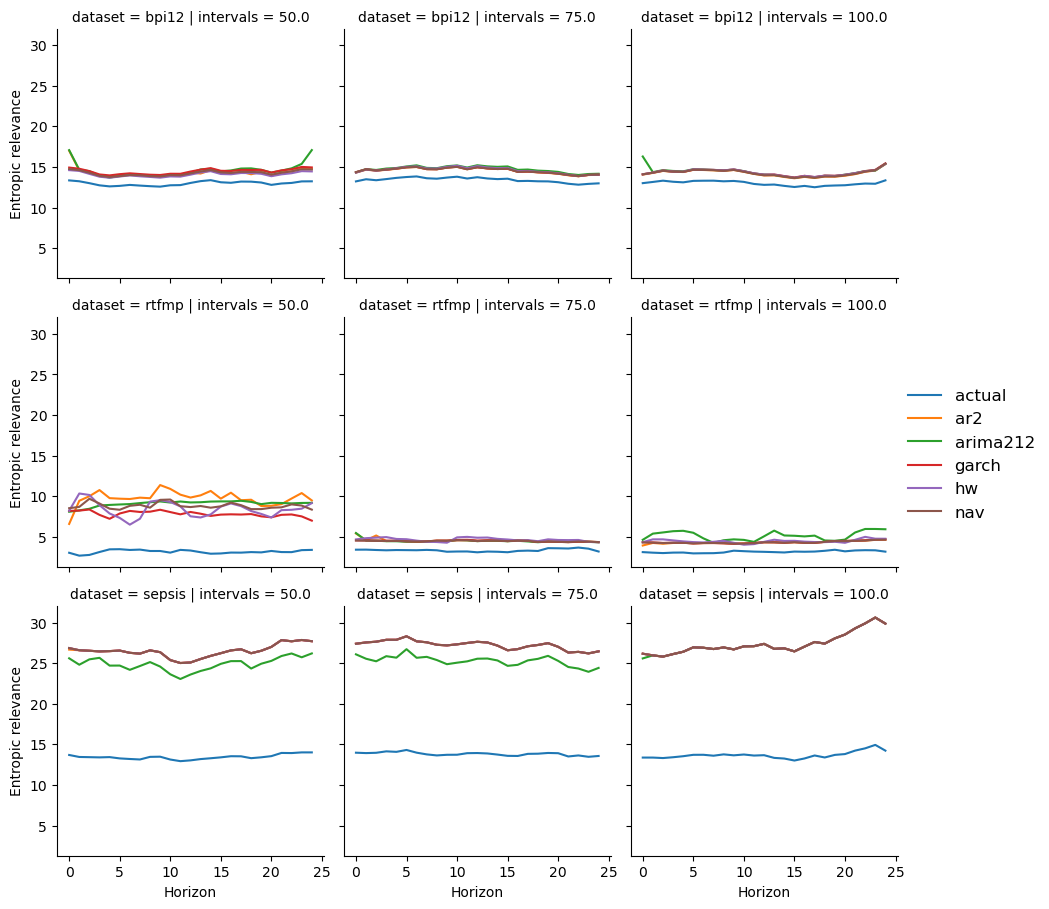
\includegraphics[width=0.8\textwidth]{img/cv_entropic_small_equisize.png}
%     % 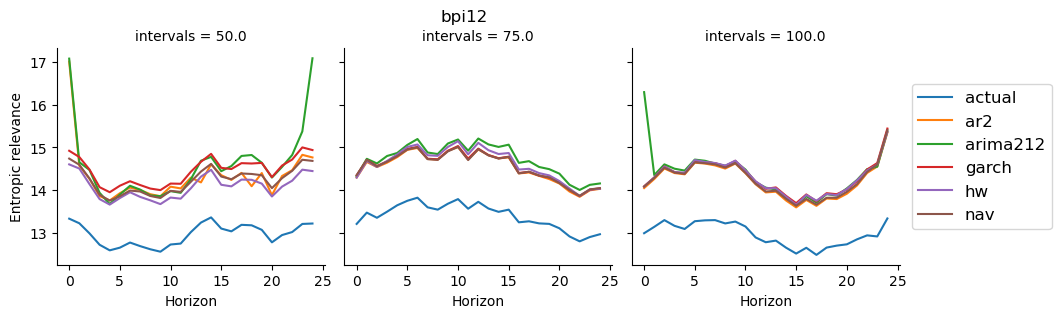
\includegraphics[width=0.8\textwidth]{img/cv_bpi12_entropic_small_equisize.png}
%     % 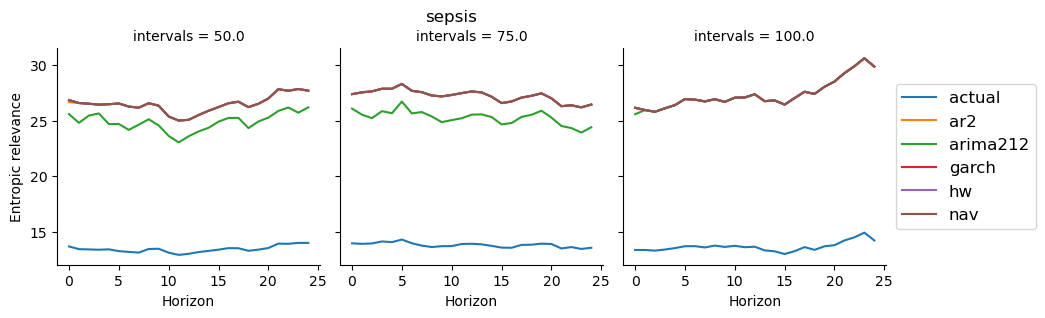
\includegraphics[width=0.8\textwidth]{img/cv_sepsis_entropic_small_equisize.png}
%     % 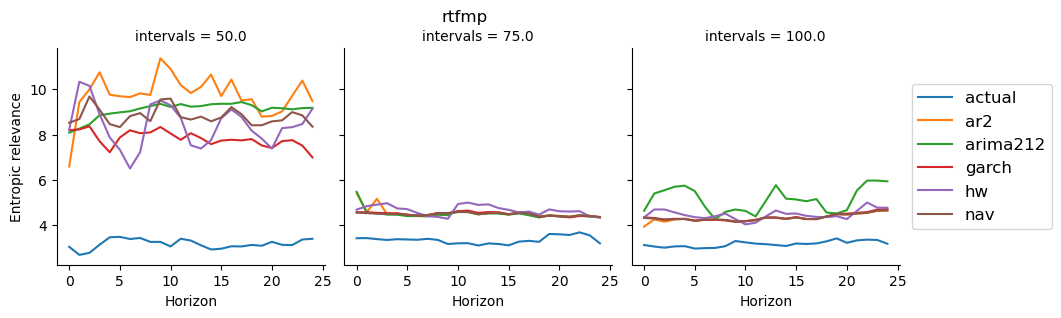
\includegraphics[width=0.8\textwidth]{img/cv_rtfmp_entropic_small_equisize.png}
%     \caption{Entropic relevance results for equisize aggregation. Best (lowest) results are indicated in bold.}
%     \label{fig:equisize}
% \end{figure}
% \begin{figure}
%     \centering
%     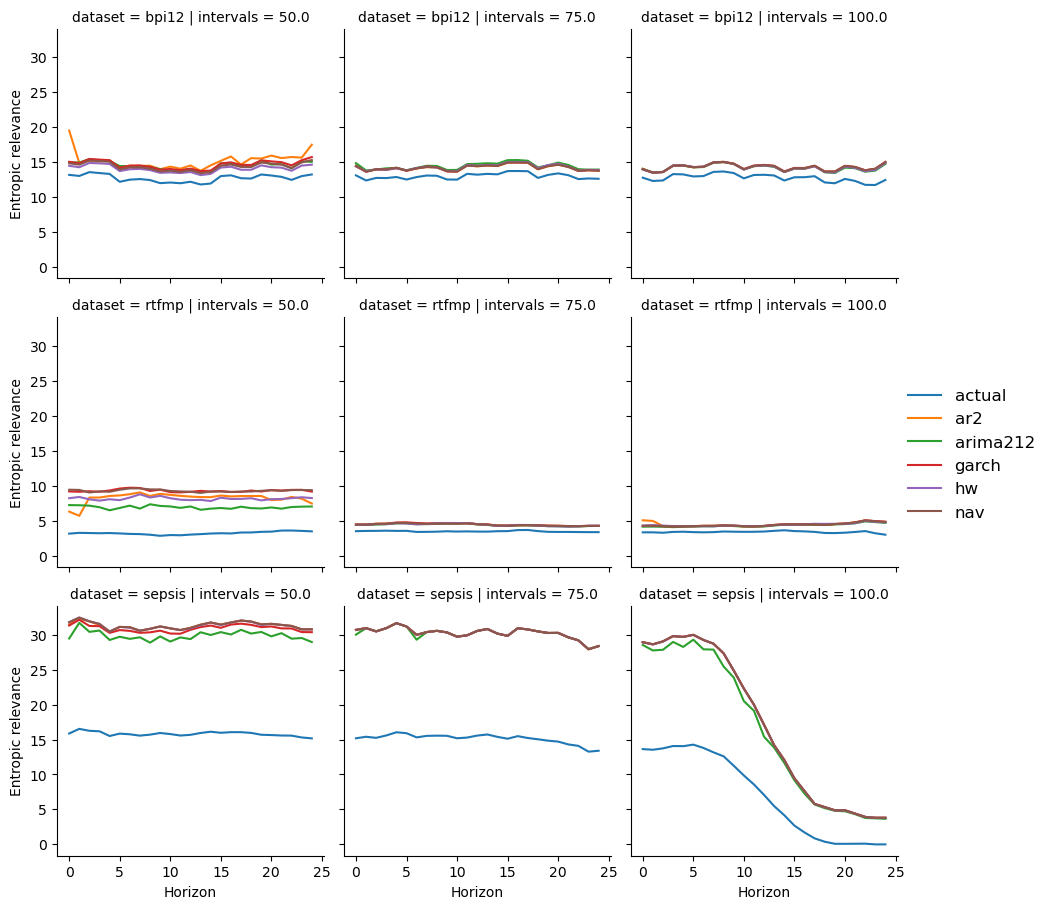
\includegraphics[width=0.8\textwidth]{img/cv_entropic_small_equitemp.png}
%     % 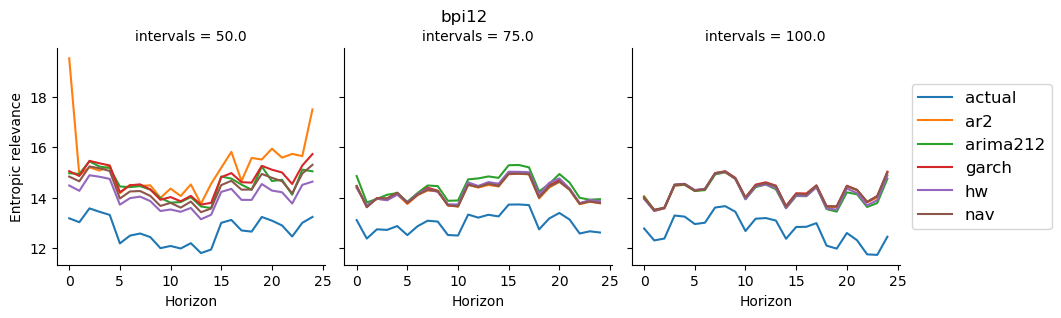
\includegraphics[width=0.8\textwidth]{img/cv_bpi12_entropic_small_equitemp.png}
%     % 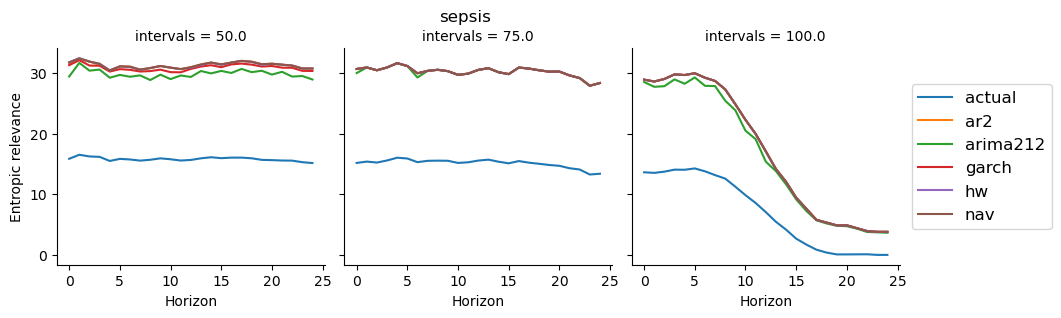
\includegraphics[width=0.8\textwidth]{img/cv_sepsis_entropic_small_equitemp.png}
%     % 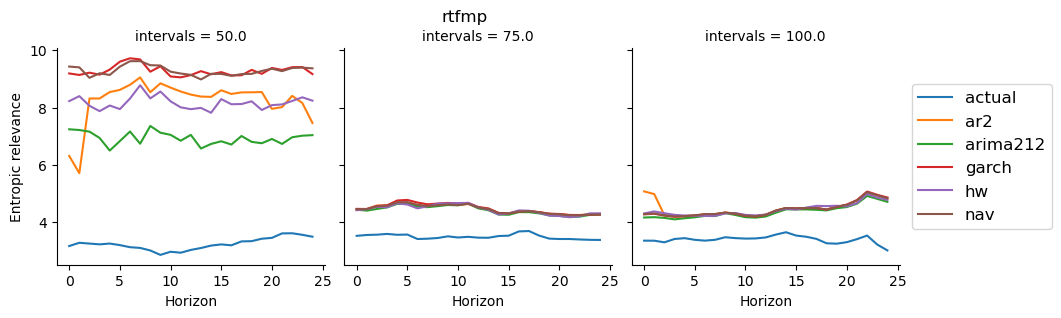
\includegraphics[width=0.8\textwidth]{img/cv_rtfmp_entropic_small_equitemp.png}
%     \caption{Entropic relevance results for equitemporal aggregation. Best (lowest) results are indicated in bold.}
%     \label{fig:equitemp}
% \end{figure}

% \subsection{Managerial implications}
% Depending on the event log, it is feasible to obtain good (\textless15\%) to very good (\textless5\%) forecasting results in terms of the MAPE and entropic relevance against actual DFGs.
% The experiments show that the number of intervals used for training vastly impacts results, which is expected given that with 10-fold cross-validation, this results in only 15 interval being used for the tenth fold to predict the next 25 intervals.
% Given that GARCH models often perform strongly suggests that DF time series benefit from the use of models which allow for a varying level of variance.
% This makes sense in an event log context, as activities generating the DF occurrences do not occur uniformly during the execution of a process.

\subsection{Visualising Process Model Forecasts}\label{sec:visualisation}

In~\Cref{sec:4.3:results} we evaluated forecasting results, ensuring the conformance and interpretability of the predicted process models. To that end, gaining actual insights from such predicted data remains a difficult task for the analyst. This section sets off to present the implementation of a novel visualisation system to aid analysts in exploration of the event logs. The process of designing and implementing the system started by designing several prototypes that undergone rounds of discussions to mature into the implemented visualisation system. 

The design of the PCE system is shown in Figure~\ref{fig:vis-two-brushes}. It shows an interactive visualisation system with several connected views. The system is implemented with D3.js JavaScript library and is available as an open source project\footnote{See \url{google.com}}.
\todo[inline]{Please check. I went to \url{google.com} and only found a search engine, but a PCE system.}

\begin{figure}
	\centering
	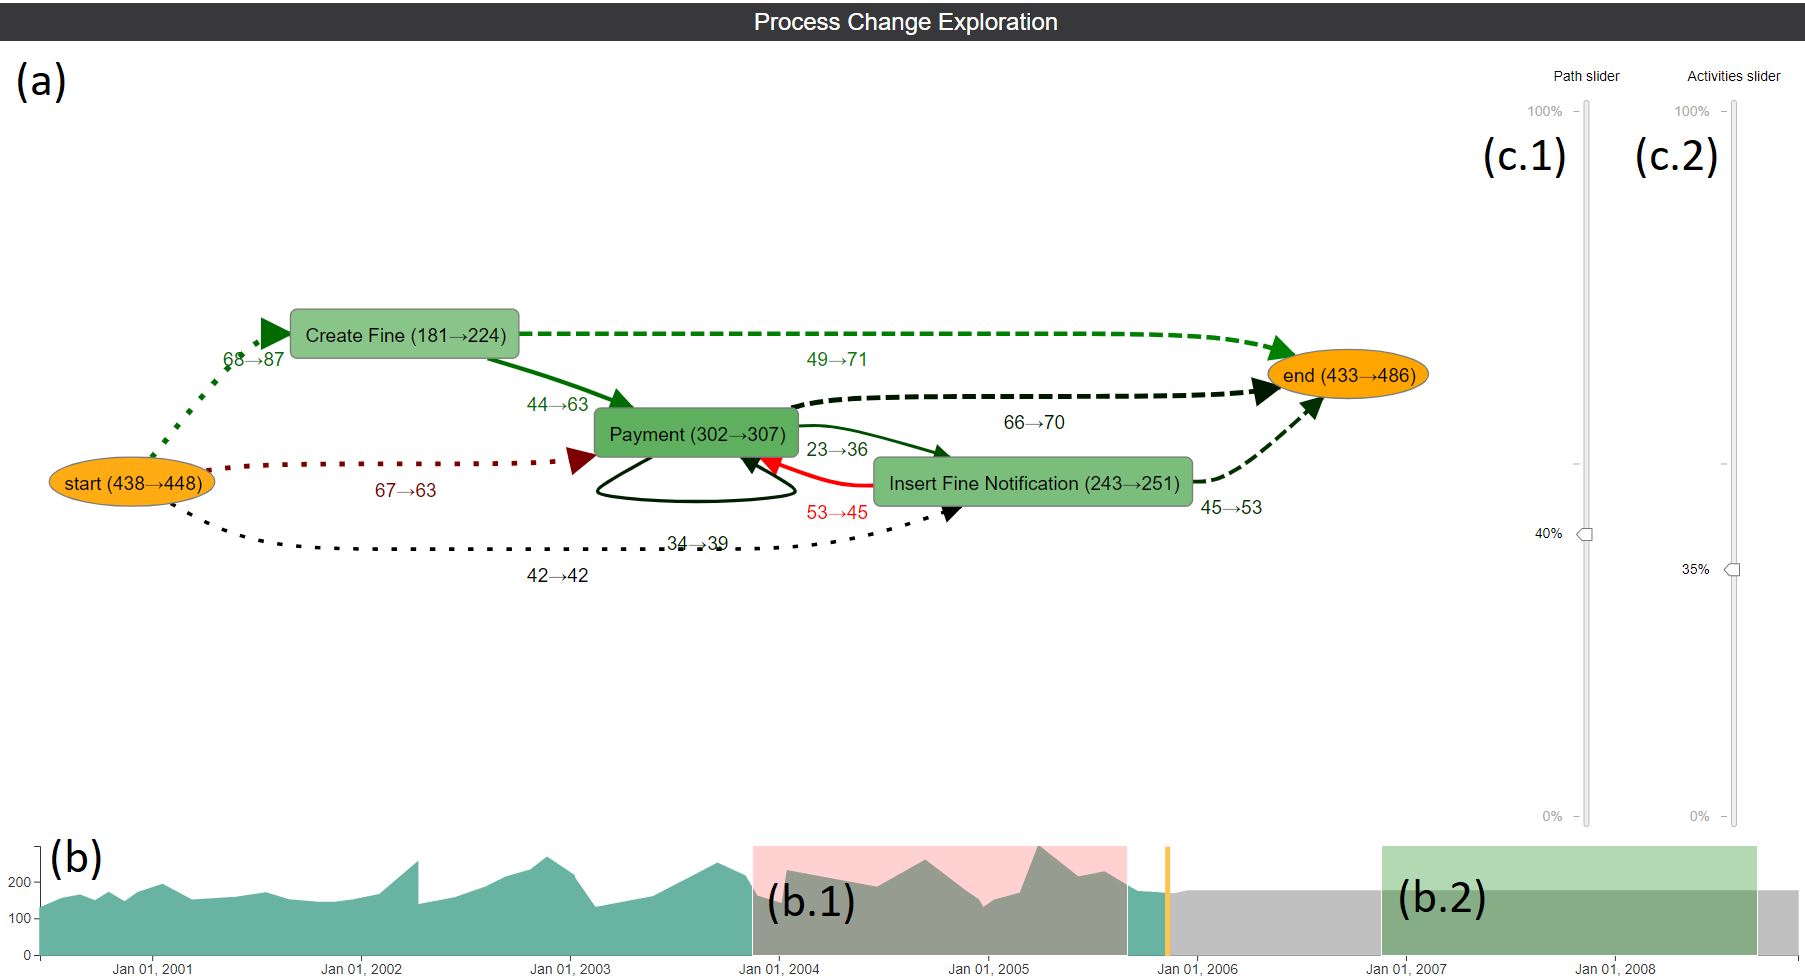
\includegraphics[width=\textwidth]{img/vis/actual-predicted-two-brushed-regions-system.PNG}
	\caption{Process Change Exploration (PCE) system.~\emph{(a)} shows~\emph{Adaptation Directly-Follows Graph (aDFG)} view.~\emph{(b)} shows the \emph{Timeline view with brushed regions} view. Users can brush one or more regions on this graph in order to filter the scope of the analysis~\emph{(b.1}, and~\emph{b.2)}. Two additional views on~\emph{(c)} show the \emph{activity and path sliders}.} 
	\label{fig:vis-two-brushes}
\end{figure}